
\clearpage
\memoto{Mr. George R. R. Martin}
\memofrom{Dragon lovers}
\begin{memo}[Memorandum]
Dear Mr. George R.R. Martin,

Thank you for this opportunity to write to express our love for your work and our thoughts on the dragon in the book. We learned that your novel \emphi{A Song of Ice and Fire} is set in medieval Europe, so we have a bold idea: if you put your story on the stage today, the dragon in the book will live in the current environment, what kind of impact it will have. We've come up with some analysis that we hope will help you maintain a realistic ecological basis for your story.

As far as we know, there has never been anything in nature like what we define as ``dragon'' today. We guess your question might be: ``the dragon's flame how to realize'', ``dragon daily activity and the energy consumption'', ``the movement of dragons from arid regions to temperate regions and arctic regions''.

In books, dragons are fire-breathing animals, and we can't get a direct reference from reality. Currently, there is no known animal in nature can spray fire, some of the so-called ``breath fire'' are just fluorescent chemicals. We take inspiration from the rumen digestion of ruminants: ruminants such as cattle and sheep can convert cellulose to methane through the rumen, even though the methane produced by these animals is excreted. In our scenario, dragons have a digestive mechanism similar to that of ruminants, producing methane and storing it in an organ of the body.(for this reason, the dragon's diet should include plants to get the cellulose needed to break down methane.)  When the dragon needs to breathe fire, the methane stored in its body is transported to its lower jaw, where it is exhaled through friction and high-speed exhalation, and then burned in the air, creating a jet of flame. Therefore, you should add some vegetables to the dragon's diet in your novel, except lambs and calves.

The daily life of an animal is closely related to its energy consumption, and when the dragon engages in war without being influenced by human factors (as described in the novel), its daily activities are similar to those of other animals in nature, from which we can draw a reference. Some lazy animals in nature, such as the koala, spend only four hours a day on foraging, moving, cleaning and interacting with other koalas, and the rest of the day is for sleeping in trees. This is because their food is of low nutritional value and they cannot get enough energy. They can only reduce their daily energy consumption by increasing their sleep time. Large herbivores, on the other hand, must spend a lot of time eating and sleeping in order to get the energy they need to maintain their lives.

For the dragon, as a huge animal, its energy consumption is also huge, so it has to absorb a lot of food. Through analysis, we obtained a graph of the dragon's food intake. It has been estimated that an adult dragon weighing about 8t would need to eat about 13.5 sheep and 808.26kg of vegetables a day. So in your book, dragons can no longer be described as unbridled gluttons, they should eat a balanced diet every day, reasonable distribution of nutrition. In order to describe the daily activities of the dragon, we also introduced the concept of mental state, which describes the changes of the dragon's energy with time. The sleep of the dragon will supplement it every night, and it will slowly wear out during the daily activities. As you can see from the picture, it describes the general activity of the dragon during the day. For reference, you can set the schedule for the dragon in the book.

Like many birds, dragons will migrate. But unlike other birds that migrate to adapt to climate, we think that because of the spirituality of the dragon, its migration model is essentially random. Because of its extremely fast speed and long flying range, the dragon covered a very wide area during its migration. So it moves from arid regions to temperate regions, to the arctic. But at the same time we consider the influence of environmental energy density and interaction between dragons in this model. Through the program simulation, the migration route of the dragon is obtained. During the migration process of the dragon, it will reach the environment with different climatic conditions due to the randomness of movement. However, due to the limitation of environmental tolerance, it will spend less time in the harsh environment and more time in the comfortable environment. A dragon is never an animal that stays put. You can better describe the migration of a dragon based on the picture.

Thank you again for taking the time to read our suggestions. We sincerely hope that the models we built can help with maintaining the realistic ecological underpinning of the story!

\hfill Sincerely,

\hfill Dragon lovers

\begin{center}
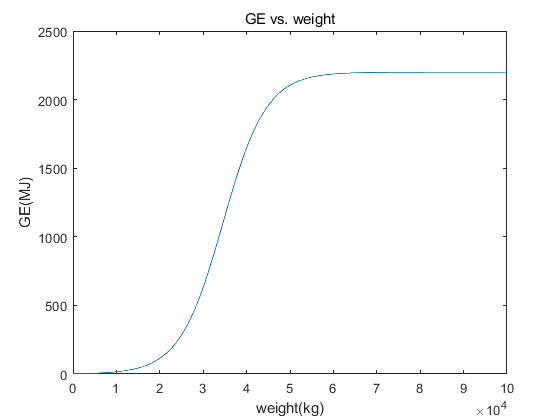
\includegraphics[width=.4\textwidth,height=.25\textwidth]{final/final1.png}
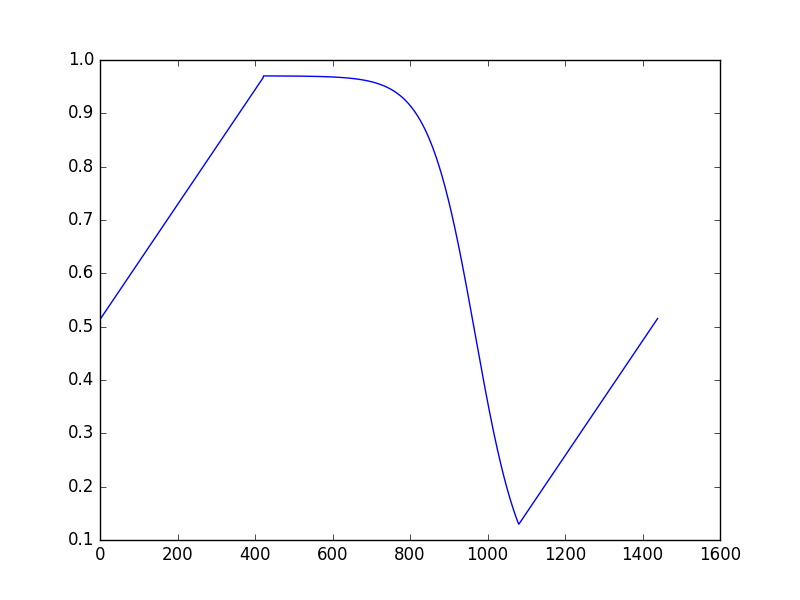
\includegraphics[width=.4\textwidth,height=.25\textwidth]{figures/attri/spirit.png}
\end{center}

\begin{center}
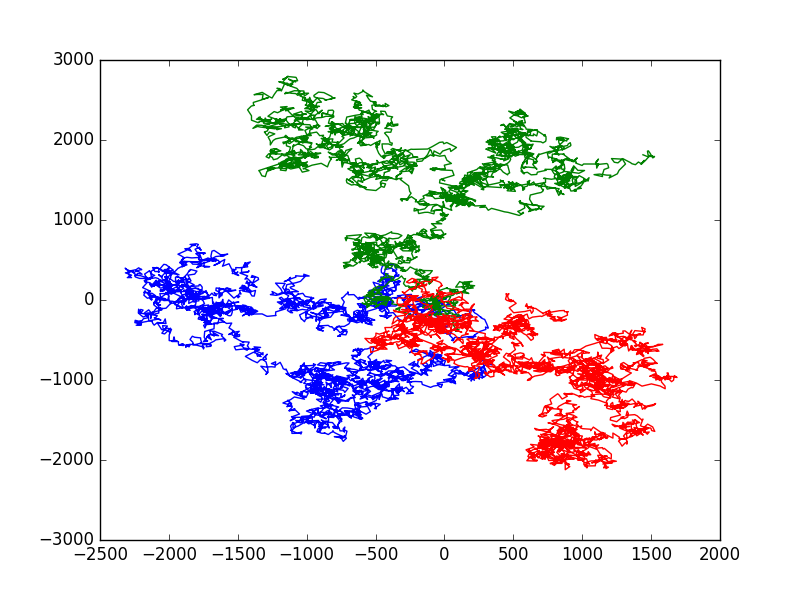
\includegraphics[width=.4\textwidth,height=.25\textwidth]{figures/interact/way.png}
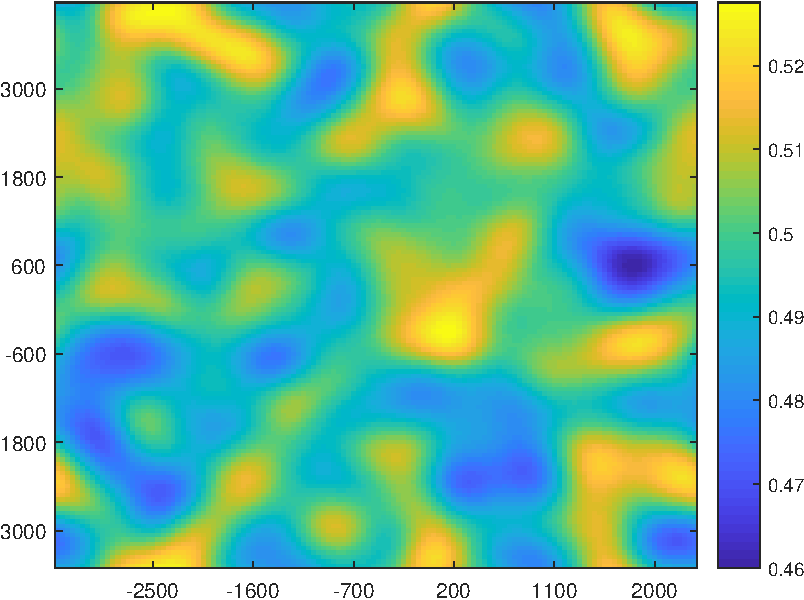
\includegraphics[width=.4\textwidth,height=.25\textwidth]{figures/interact/env.pdf}
\end{center}

\end{memo}
